% Created 2012-09-20 Thu 17:18
\documentclass[11pt]{article}
\usepackage[utf8]{inputenc}
\usepackage[T1]{fontenc}
\usepackage{fixltx2e}
\usepackage{graphicx}
\usepackage{longtable}
\usepackage{float}
\usepackage{wrapfig}
\usepackage{soul}
\usepackage{textcomp}
\usepackage{marvosym}
\usepackage{wasysym}
\usepackage{latexsym}
\usepackage{amssymb}
\usepackage{hyperref}
\tolerance=1000
\providecommand{\alert}[1]{\textbf{#1}}

\title{ZhangBank}
\author{Ian Logan, Cameron Lopez, Anton Moczygemba, Isaac Noojin}
\date{\today}
\hypersetup{
  pdfkeywords={},
  pdfsubject={},
  pdfcreator={Emacs Org-mode version 7.8.11}}

\begin{document}

\maketitle


\section*{Description}
\label{sec-1}


  Our application seeks to fill needs of students
  everywhere. ZhangBank's goal is to organize a class's material
  collectively. Students can upload lectures, notes, and study guides,
  whatever can help the class rise up and meet the expectations of
  their professors.

  Identifiable entities include user accounts, roles, documents (of
  many kind), document types, courses, professors, and semesters. An
  organized way to find and view documents will be implemented, as
  well as add content. A user profile will keep track of which courses
  students are taking or are interested in. An nteresting problem
  would be correctly displaying each arbitrary document. Data for our
  application can be generated from our own courses and other free
  online courses.
  
\subsection*{\textbf{TODO} - Isaac}
\label{sec-1-1}

   Clean up this description. Some on what I described should go in
   design section. Read the instructions for ``General Description of
   Application Domain'' of what to hand in and make sure it has
   everything required and is clear and consise. If you have any
   questions about what our project is (a better FreeTestBank.com),
   ask.
\section*{Design}
\label{sec-2}
\subsection*{\textbf{TODO} - Anton, Cameron, Ian, Isaac}
\label{sec-2-1}

   Lets get down what we want our project to do. Write it down, type
   it up, doesn't matter. Just get it to me somehow. We'll need to
   decide what we want to implement so we can start desining our
   schema

\begin{itemize}
\item Functionality
\item Types of users
\begin{itemize}
\item Functionality of each role
\end{itemize}
\end{itemize}
\section*{Schema}
\label{sec-3}


  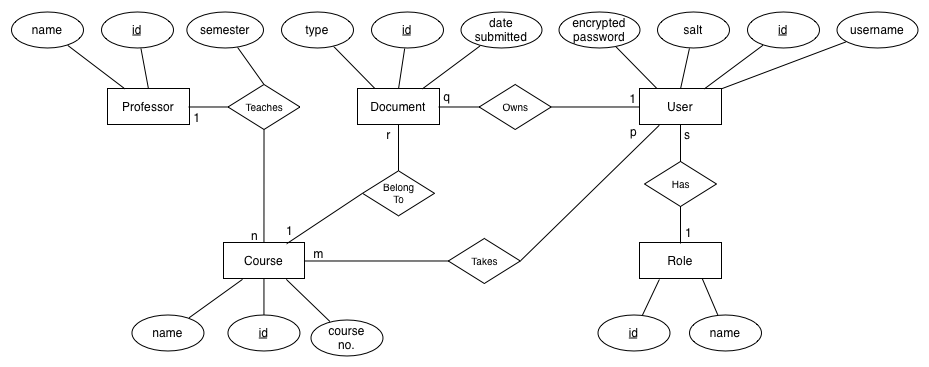
\includegraphics[width=.9\linewidth]{ER Diagram.png}
\subsection*{\textbf{TODO} - Finish Design}
\label{sec-3-1}

   E/R diagram

\end{document}